\documentclass[tikz,border=4pt]{standalone}
\usepackage{tikz}
\usetikzlibrary{arrows.meta,calc}
\definecolor{nebula}{HTML}{6366F1}
\definecolor{spark}{HTML}{14B8A6}
\begin{document}
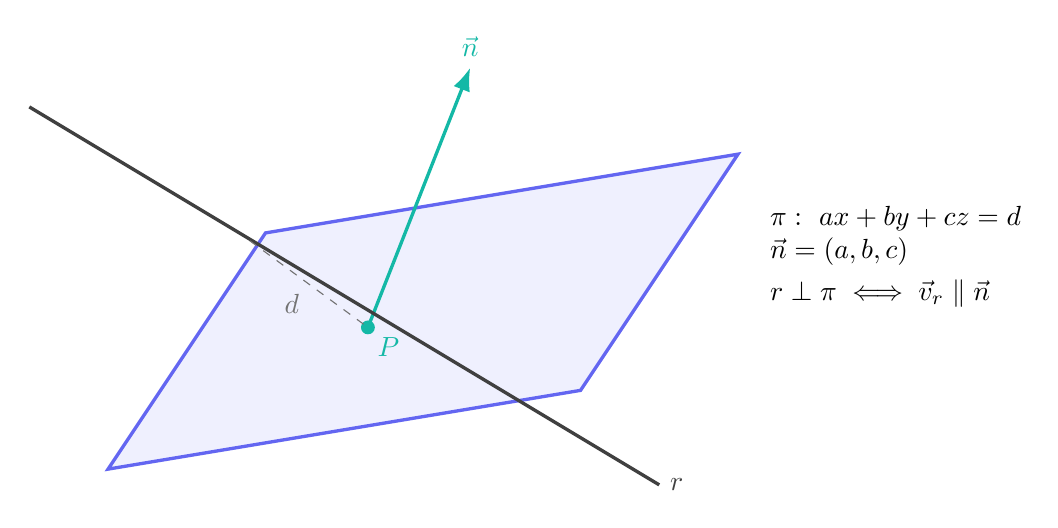
\begin{tikzpicture}[font=\sffamily,>=Latex]
  \coordinate (A) at (0,0); \coordinate (B) at (6,1); \coordinate (C) at (8,4); \coordinate (D) at (2,3);
  \fill[nebula!10] (A)--(B)--(C)--(D)--cycle;
  \draw[nebula,very thick] (A)--(B)--(C)--(D)--cycle;
  \fill[spark] (3.3,1.8) circle (2.5pt) node[below right] {$P$};
  \draw[->,very thick,spark] (3.3,1.8)--(4.6,5.1) node[above] {$\vec n$};
  \draw[very thick,black!75] (-1,4.6)--(7,-.2) node[right] {$r$};
  \draw[dashed,black!55] (1.8,2.9)--(3.3,1.8) node[midway,below left] {$d$};
  \node[align=left] at (10,2.7) {$\pi:\ ax+by+cz=d$\\$\vec n=(a,b,c)$\\[3pt]$r\perp\pi\iff\vec v_r\parallel\vec n$};
\end{tikzpicture}
\end{document}
